\documentclass[10pt]{article}
\usepackage{neurips_lite}
\setcitestyle{numbers,round,sort&compress}
\usepackage{amsmath,amssymb}
\usepackage{graphicx}
\usepackage{booktabs}
\usepackage{microtype}
\setlength{\emergencystretch}{1em}
\usepackage{xcolor}
\usepackage[colorlinks=true,linkcolor=blue!60!black,citecolor=blue!60!black,urlcolor=blue!60!black]{hyperref}

\newcommand{\coverage}{C}
\newcommand{\repetition}{R}
\newcommand{\groktime}{GrokTime}
\newcommand{\memtime}{MemTime}
\newcommand{\todo}[1]{\textbf{\textcolor{red}{[TODO-AUTHOR: #1]}}}
\newcommand{\sugg}[1]{\textbf{\textcolor{purple}{[SUGGESTED - AUTHOR MUST VERIFY: #1]}}}

% Title applied per author decision (alternative 1). Unused alternatives retained for reference;
% delete this comment before submission:
% (2) Data coverage, not within-epoch repetition, gates grokking at matched per-example dose
% (3) Unique coverage gates generalization in transformer grokking: within-epoch repetition shows no detectable effect at matched dose
\title{Coverage versus within-epoch repetition at matched dose in transformer grokking}

\author{Chang Tan\\
Dalian University of Technology, Dalian, China\\
\texttt{aquars43@foxmail.com}}
% TODO-AUTHOR: add school/department and postal code within Dalian University of Technology
% if the Neural Processing Letters title-page format requires them (sole author; corresponding author).

\begin{document}
\maketitle

\begin{abstract}
How much of a neural network's generalization comes from unique training data, and how much from seeing the same data again? We separate the two levers in a controlled grokking setup. A two-layer transformer ($1.04\times10^{5}$ parameters) learns modular addition ($p=23$; 529 unique problems), with training-set coverage (25--85\% of all problems), within-epoch repetition ($R \in \{1,2,4,8\}$), and the arrangement of repeated copies (blocked versus interleaved) manipulated in a partially crossed design (27 conditions, 5 seeds each, 135 runs), while a continuous batching scheme holds the expected per-example dose identical across $R$. Coverage dominates: median GrokTime, the first step at which test accuracy reaches 95\%, falls from $8{,}400$ steps at 45\% coverage to $1{,}800$ at 85\% (rank-biserial $r=+1.0$, Holm-adjusted $p=0.016$; permutation log-rank $p=0.008$); at 35\% coverage only three of thirty-five runs generalize, and at 25\% none do within the $20{,}000$-step budget. Repetition shows no detectable effect on GrokTime at matched per-example dose, with every confidence interval including zero, but it is not without effect: it delays memorization (MemTime, the first step at which training accuracy reaches 95\%, rises from 100 to 300 steps at 55\% coverage between $R=1$ and $R=8$), raises sub-critical final accuracy at 25\% coverage ($13.4\%$ to $21.7\%$ between $R=1$ and $R=4$), and sustains larger final weight norms there. In this regime, under a fixed optimization budget and at matched per-example dose, unique coverage rather than repeated exposure governs the transition from memorization to generalization.
\end{abstract}

\noindent\textbf{Keywords:} Grokking; Data coverage; Data repetition; Data-constrained training; Transformers; Generalization

\section{Introduction}

Neural networks can memorize their training data long before they generalize. On modular arithmetic tasks, a transformer fits a mid-sized training set within a few hundred steps, yet test accuracy can remain near chance for thousands of steps longer before an abrupt transition to near-perfect generalization \citep{power2022grokking}. This delay, called grokking, is not specific to tiny models: the same tension between memorizing individual items and computing a rule underlies practical questions about deduplication, repetition, and data-constrained pretraining of large language models \citep{lee2022deduplicating, muennighoff2023scaling, allen-zhu2024physics}.

Both literatures, however, tend to treat training data as a scalar quantity. ``How much data'' conflates two decisions that practitioners make separately: \emph{coverage}, the number of distinct examples the training set spans, and \emph{repetition}, how often each example is seen. The dependence of grokking on dataset size is itself well documented: delayed generalization appears only within a range of dataset fractions \citep{power2022grokking}, varies strongly with the number of unique training items \citep{liu2023omnigrok}, and is predicted by circuit-efficiency accounts to require a sufficient supply of unique examples for the generalizing circuit to dominate \citep{varma2024explaining}. What prior work does not isolate is repetition as a separate factor: at a matched optimization budget, does it matter how often each unique example is shown, or in what arrangement those exposures arrive? At the scale of language models, coverage and repetition are entangled with corpus composition, tokenizer statistics, and stopping points; at the scale of grokking studies, the two have not been separated.

This paper provides such a separation in a system small enough to be exactly characterized. A two-layer transformer learns modular addition, $(a+b) \bmod 23$, a task with exactly 529 unique problems. We vary the coverage of the training set ($\coverage \in \{25,35,45,55,70,85\}\%$ of all problems, tested on the held-out complement), the within-epoch repetition of each example ($\repetition \in \{1,2,4,8\}$), and the arrangement of the repeated copies: \emph{blocked} (copies adjacent, as in near-duplicate documents) or \emph{interleaved} (uniformly reshuffled, as in multi-epoch training). The design is partially crossed rather than fully factorial (Sect.~\ref{sec:design}); it comprises 27 conditions with 5 seeds each (135 runs). Batches are drawn from a continuous stream so that every optimization step consumes exactly 256 examples in every condition; at matched steps, the expected per-example dose is identical across $\repetition$ within a coverage level, so $\repetition$ isolates the temporal clustering of repeated exposures. Analysis is at the seed level, with explicit right-censoring at the step budget.

Three findings emerge. First, coverage gates the transition: median GrokTime falls monotonically from $8{,}400$ steps at $\coverage{=}45\%$ to $1{,}800$ at $\coverage{=}85\%$ (rank-biserial $r=+1.0$, exact permutation $p=0.008$, Holm-adjusted $p=0.016$; permutation log-rank $p=0.008$), while below roughly $35\%$ coverage generalization becomes unreliable and at $25\%$ no seed generalizes within budget despite immediate memorization. Second, at matched per-example dose, repetition shows no detectable effect on GrokTime in either arrangement: the declared contrasts give point estimates of at most $900$ steps, every confidence interval includes zero, and the censoring-aware analyses (permutation log-rank, restricted mean survival time, a stratified Cox model) agree. This is a null result bounded by the design, not evidence of exact equivalence. Third, repetition does leave detectable traces on secondary outcomes: it slightly delays memorization, raises sub-critical final accuracy below the coverage boundary, and sustains larger final weight norms, a pattern consistent with repetition supporting the memorizing solution rather than accelerating generalization. A single-seed pilot observation that blocked repetition accelerated the transition did not replicate across seeds; we report this as a caution for single-seed grokking studies.

Our contribution is threefold: (i) a matched-budget, partially crossed design that separates coverage from within-epoch repetition and its arrangement at the level of individual examples; (ii) seed-level, censoring-aware statistics showing that coverage gates whether and when generalization occurs (85\% vs.\ 45\% coverage: median GrokTime difference $-6{,}600$ steps, 95\% CI $[-11{,}600, -4{,}000]$, Holm-adjusted $p=0.016$; three of thirty-five runs generalize at 35\%, none at 25\%), reproducing the known dataset-fraction dependence at higher evidential resolution; and (iii) a bounded null result on repetition at matched dose, with the detectable secondary effects reported alongside rather than smoothed over.

\section{Related work}

\paragraph{Delayed generalization.}
Grokking, the rapid memorization of a small training set followed by an abrupt transition to near-perfect test accuracy long after overfitting, was characterized on modular arithmetic tasks, where it appears only within a narrow range of dataset fractions and optimization settings \citep{power2022grokking}. Subsequent work explained the transition through loss-landscape geometry and weight norms \citep{liu2023omnigrok}, mechanistic progress measures that change smoothly before test accuracy jumps \citep{nanda2024progress}, and circuit efficiency, under which generalizing solutions are parameter-efficient but slower to learn than memorizing ones \citep{varma2024explaining}. These studies manipulate how much unique data the model sees; the count and arrangement of repeated exposures at matched budget has not been treated as a separate factor. We build on the standard two-layer-transformer arithmetic setup \citep{power2022grokking, nanda2024progress} and hold the optimization budget fixed while decomposing the data axis into coverage and repetition.

\paragraph{Data-constrained pretraining and repetition.}
As high-quality text becomes scarce, repeating data has become routine practice. Repeating a corpus for up to roughly four epochs changes loss little, while more epochs degrade returns \citep{muennighoff2023scaling}; compute-optimal scaling laws allocate budget between model size and tokens \citep{kaplan2020scaling, hoffmann2022training}; and complementary work measures memorization directly: networks can fit random labels \citep{zhang2017understanding}, knowledge capacity scales with parameters and repeats \citep{allen-zhu2024physics}, and deduplication reduces verbatim recall \citep{lee2022deduplicating}. Ordering effects among unique examples (curricula) have mixed consequences, with benefits concentrated in noisy or time-varying regimes \citep{wu2021curricula, bengio2009curriculum}. These results are obtained at scale, where unique coverage and repetition count are entangled with tokenizer statistics, corpus composition, and stop-point confounds; controlled, seed-level evidence at matched optimization steps is missing. Our design supplies it in a system where every training item, exposure count, and evaluation point is exactly tracked.

\paragraph{Positioning.}
Two prior findings bracket our results. On critical dataset size, reduced training fractions are known to delay or prevent grokking \citep{power2022grokking, liu2023omnigrok, varma2024explaining}. On repeated data, multi-epoch repetition at pretraining scale is known to be nearly free for a few epochs and costly beyond \citep{muennighoff2023scaling, allen-zhu2024physics}. The present work is complementary to both lines: it reproduces the coverage dependence at seed level with censoring-aware statistics, and adds what neither line provides, namely a within-coverage manipulation of repetition count and arrangement at matched per-example dose.

\section{Methods}

\subsection{Task, model, and optimization}
\label{sec:task}

We study modular addition, $(a+b) \bmod p$ with $p=23$, which admits exactly $p^2=529$ distinct problems. Each problem is a four-token causal sequence $[a, \texttt{+}, b, \texttt{=}]$; the model predicts the answer token at the final position, and the answer never appears in the input. The learner is a two-layer causal transformer \citep{vaswani2017attention} with model dimension 64, four attention heads, and a fourfold multilayer perceptron (MLP) expansion ($1.04\times10^{5}$ parameters). We optimize with AdamW \citep{loshchilov2019decoupled} at learning rate $10^{-3}$, $\beta=(0.9,0.98)$, and weight decay $1.0$ on all parameters, following the configuration under which delayed generalization was originally characterized \citep{power2022grokking, nanda2024progress}. Each step consumes exactly $B=256$ examples; the budget is $20{,}000$ steps per run; test accuracy is evaluated every 100 steps on the held-out complement of the training set. All experiments ran on CPU; a full run takes 1--10 minutes.

\subsection{Data stream: coverage and repetition as separate factors}
\label{sec:stream}

A run is configured by three factors. \emph{Coverage} $\coverage \in \{25,35,45,55,70,85\}\%$ fixes the number of unique training examples, $n_{\mathrm{uniq}} = \mathrm{round}(\coverage \cdot 529)$ (450 at 85\%, 291 at 55\%, 132 at 25\%), sampled once per seed; the remaining problems form the disjoint test set (79 held-out problems at 85\% coverage, 238 at 55\%, 397 at 25\%). \emph{Repetition} $\repetition \in \{1,2,4,8\}$ fixes how many copies of each unique example one epoch of the training list contains. \emph{Mode} controls the arrangement of the copies: under \emph{blocked} repetition the $\repetition$ copies are adjacent (the unique order is reshuffled each epoch); under \emph{interleaved} repetition the full list of $n_{\mathrm{uniq}} \cdot \repetition$ entries is reshuffled uniformly. For $\repetition = 1$ the two modes coincide and serve as the shared baseline.

Batches are drawn from a continuous stream across epoch boundaries, so every step consumes exactly 256 examples in every condition. At a fixed number of steps $T$, the expected number of exposures of each unique example is $BT/n_{\mathrm{uniq}}$, which is independent of $\repetition$; the total number of gradient updates and the expected per-example dose are therefore matched across $\repetition$ within a coverage level. Two consequences follow, and we state them explicitly because they define what the experiment tests. First, with 256 examples per step drawn from a continuously reshuffled multiset, interleaved repetition is close to sampling with replacement from the unique set; an effect of repetition count per se is expected to be small in this arm. Second, blocked repetition concentrates copies in time, in particular within batches: at $\repetition=8$ a batch can contain as few as 32 unique problems, versus up to 256 at $\repetition=1$. The blocked-versus-interleaved contrast therefore mainly tests the temporal clustering of repeated exposures and the associated within-batch duplication, not the effect of additional exposure, which is excluded by construction. The experiment does not test unmatched-dose repetition (the practical regime in which more repetition buys more updates), and it does not separate within-batch diversity from temporal clustering; a batch-size control would be needed for the latter. Coverage, in contrast, simultaneously changes the number of distinct problems and the per-example dose at fixed budget, mirroring the practical trade-off between more unique data and more passes over fewer unique data \citep{muennighoff2023scaling}.

\subsection{Design}
\label{sec:design}

The design is partially crossed, not a full factorial of coverage, repetition, and mode. Table~\ref{tab:design} lists the cells. The $R=1$ baseline spans all six coverage levels (arm A). Blocked and interleaved repetition are crossed with coverage only at $\{35,55,85\}\%$ (arms B and C). A sub-critical arm at 25\% coverage (arm D: blocked $R \in \{4,8\}$ and interleaved $R=8$) was added when the initial run list was found to omit a cell required by the declared extreme contrast; the addition was decided after arm-A results were known and before any arm-D data were collected, and is logged in Appendix~B. In total the design comprises 27 conditions, 5 seeds per condition, 135 runs.

\begin{table}[t]
\centering
\caption{\textbf{Partially crossed design.} Cells actually run, with the number of conditions and runs (5 seeds per condition). Mode is vacuous at $R=1$; the $R=1$ baseline is shared between modes.}
\label{tab:design}
\small
\begin{tabular}{llllrr}
\toprule
Arm & Coverage (\%) & $R$ & Mode & Conditions & Runs \\
\midrule
A & 25, 35, 45, 55, 70, 85 & 1 & shared baseline & 6 & 30 \\
B & 35, 55, 85 & 2, 4, 8 & blocked & 9 & 45 \\
C & 35, 55, 85 & 2, 4, 8 & interleaved & 9 & 45 \\
D & 25 & 4, 8 & blocked & 2 & 10 \\
D & 25 & 8 & interleaved & 1 & 5 \\
\midrule
\multicolumn{3}{l}{Total} & & 27 & 135 \\
\bottomrule
\end{tabular}
\end{table}

\subsection{Outcomes and statistical analysis}
\label{sec:outcomes}

The independent experimental unit is the random seed, which jointly controls parameter initialization, the choice of the unique training subset, and data order; $n=5$ seeds (0--4) per condition. Training curves within a run are repeated measurements and are never treated as independent. The exclusion criterion was fixed before the main runs (non-finite loss, or training accuracy below 1\% at budget exhaustion); no run met either criterion, so all 135 runs enter the analysis.

The primary outcome is \groktime{}: the first evaluation step at which test accuracy reaches at least 95\%. Runs that never reach this threshold within 20{,}000 steps are right-censored. A run stops at the first evaluation step where the criterion is met; consequently, for grokked runs the final test accuracy is the value at the stopping step, and for censored runs it is the value at budget exhaustion. Secondary outcomes are \memtime{} (the first step at which training accuracy reaches at least 95\%), final test accuracy, and the final parameter $\ell_2$ norm; the norm trajectory was a pre-specified exploratory outcome motivated by loss-landscape analyses \citep{liu2023omnigrok}. Because accuracy is evaluated every 100 steps, \groktime{} and \memtime{} are resolved to 100 steps and heavily tied within cells; medians of five such values are coarse, and the confidence intervals around them should be read as indicative.

We report medians with interquartile ranges (IQRs) across seeds and show all individual runs. The primary comparisons form three families with Holm correction within each; the families differ from the internal plan and are therefore declared rather than pre-specified (deviation-log item iii): coverage contrasts at $R=1$, blocked-repetition contrasts at matched coverage, and the extreme contrast of Sect.~\ref{sec:below}. Two-sample comparisons use the exact permutation Mann--Whitney test: all $\binom{10}{5} = 252$ label assignments are enumerated, with midranks for ties, and the two-sided $p$-value is the proportion of assignments whose $|U - n_1 n_2 / 2|$ is at least as large as the observed one. The rank-biserial effect size is $r = 1 - 2U_1/(n_1 n_2)$, where $U_1$ counts cross-group pairs in which the first-named run has the larger value, so $r = +1$ indicates that every first-named run is smaller than every second-named run; the median difference is reported as first-named minus second-named condition. Median differences carry percentile-bootstrap 95\% confidence intervals (CIs; 10{,}000 within-group resamples, fixed random seed); with five tied, 100-step-resolution values per group these intervals are coarse by construction, and the exact two-sided $p$ for a 5-versus-5 contrast cannot fall below $2/252 = 0.0079$. In rank-based \groktime{} comparisons, censored runs enter at the budget (worst rank).

Because \groktime{} is right-censored at the 20{,}000-step budget, we complement the rank tests with survival analyses that treat censoring natively: Kaplan--Meier estimates (Figs.~\ref{fig:km} and~\ref{fig:kmrep}), permutation log-rank tests (full enumeration of the 252 assignments for 5-versus-5 contrasts; 10{,}000 Monte-Carlo permutations for $k$-sample tests), and restricted mean survival time (RMST) up to the 20{,}000-step horizon with bootstrap 95\% CIs of between-condition differences, which serves as the main censoring-aware effect size. A stratified Cox proportional-hazards model additionally pools the blocked-repetition cells across the matched coverages: a single binary covariate codes blocked repetition ($R \in \{2,4,8\}$: 1) against the shared $R=1$ baseline (0), coverage level (35, 55, 85\%) is the stratification variable, and 60 runs with 43 events enter the fit. Tied event times are handled by the Breslow approximation, the partial likelihood is maximized by Newton--Raphson, the hazard ratio carries a Wald 95\% confidence interval, and the model is implemented directly in NumPy within the archived analysis pipeline (no external survival-analysis package). Cells with too few events for time-based inference are summarized by the number of runs that generalize, with Fisher exact tests and Clopper--Pearson 95\% intervals. Secondary outcomes (\memtime{}, sub-critical final accuracy, final $\ell_2$ norm, and weight norm at the matched step 1{,}000) are analyzed in separate, explicitly exploratory families, Holm-corrected within family; their $p$-values are descriptive. Monotone trends of \memtime{} across $R$ within a coverage are quantified with the one-sided (increasing-alternative) Jonckheere--Terpstra statistic, whose $p$-value is obtained from $10{,}000$ Monte-Carlo permutations of the pooled labels; rank associations use Spearman's $\rho$ with a two-sided permutation $p$-value from $10{,}000$ permutations of one variable. For the repetition contrasts in the uncensored cells (55\% and 85\% coverage) we additionally report two one-sided tests (TOST) for equivalence on $\log_{10}$ \groktime{}, with the margin expressed as a ratio. The margins were not chosen before the results were seen, so the equivalence analysis is a post hoc sensitivity analysis over the grid of margins actually run ($\pm 10\%$, $\pm 25\%$, and $\pm 50\%$; ratios 1.10, 1.25, and 1.50), and no equivalence claim is made at any margin. ``No detectable effect'' denotes a non-significant difference with interval-based bounds, not demonstrated equivalence.

The analysis was planned in an internal design document; there is no public registry entry, and the deviations from that plan are listed in Appendix~B. All resampling uses NumPy's \texttt{default\_rng} with master seed 20260922 and documented per-analysis offsets. Analyses used Python 3.12, NumPy 2.1, SciPy 1.14, and pandas 2.2; training used PyTorch 2.14 (CPU). The archived analysis pipeline, including the declared families and seed offsets, is available with the code (Declarations).

\section{Results}

\begin{figure}[t]
\centering
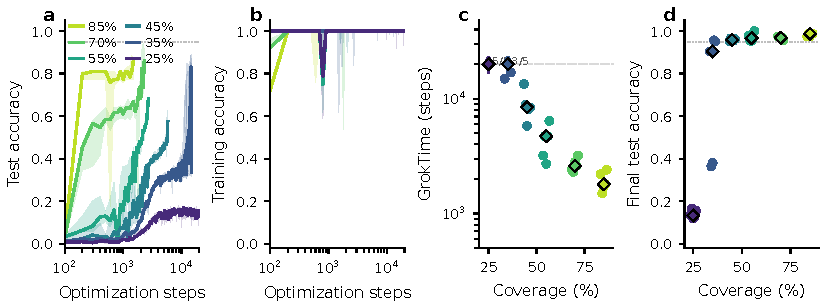
\includegraphics[width=\textwidth]{figs/fig1_coverage.pdf}
\caption{\textbf{Coverage gates the generalization transition at matched budget.} (\textbf{a}) Test accuracy versus optimization steps for the six coverage levels at $R=1$ ($n=5$ seeds per condition; lines are medians; shaded bands are interquartile ranges; the dotted line marks the 95\% generalization criterion; accuracy is evaluated every 100 steps and a run stops at the first evaluation step meeting the criterion). (\textbf{b}) Training accuracy for the same runs. (\textbf{c}) \groktime{} by coverage: points are individual seeds, filled diamonds are medians, upward arrows mark right-censored runs that did not generalize within the $20{,}000$-step budget, ``$k/5$'' gives censored runs of five, and the dashed line is the budget. (\textbf{d}) Final test accuracy by coverage (points: seeds; diamonds: medians); for grokked runs this is the value at the stopping step, for censored runs the value at budget exhaustion.}
\label{fig:coverage}
\end{figure}

\begin{figure}[t]
\centering
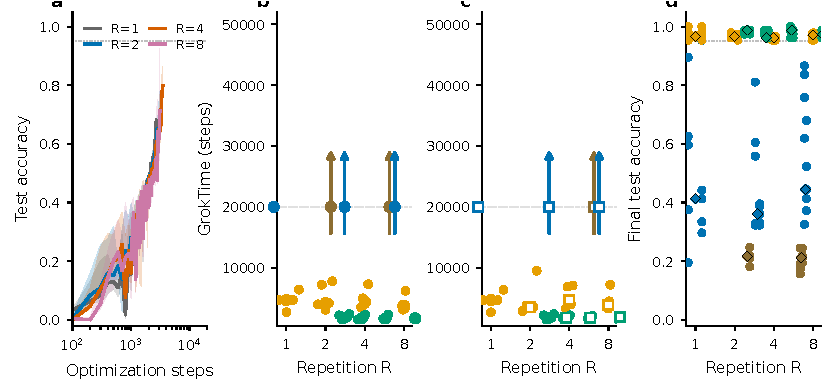
\includegraphics[width=\textwidth]{figs/fig2_repetition.pdf}
\caption{\textbf{Repetition at matched per-example dose.} (\textbf{a}) Test accuracy versus steps at $C{=}55\%$ coverage under blocked repetition with $R \in \{1,2,4,8\}$ ($n=5$ seeds per condition; lines are medians; shaded bands are interquartile ranges). (\textbf{b}) \groktime{} versus $R$ for blocked repetition at three coverage levels (points: individual seeds; filled circles: medians; upward arrows: right-censored runs within the $20{,}000$-step budget). (\textbf{c}) Same for interleaved repetition (squares: medians; censoring convention as in b). (\textbf{d}) Final test accuracy versus $R$ for both modes; for grokked runs this is the stopping value, for censored runs the value at budget exhaustion. At fixed steps the expected per-example dose is independent of $R$.}
\label{fig:repetition}
\end{figure}

\begin{figure}[t]
\centering
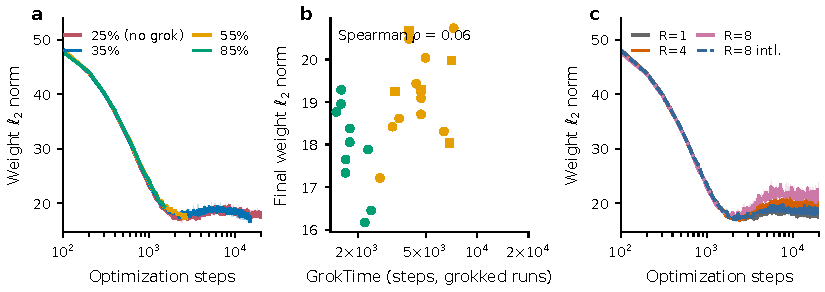
\includegraphics[width=\textwidth]{figs/fig3_wnorm.pdf}
\caption{\textbf{Weight-norm dynamics (pre-specified exploratory outcome).} (\textbf{a}) Parameter $\ell_2$ norm versus steps at $R=1$ for coverage $85\%$, $55\%$, $35\%$ (at least some seeds generalize within budget) and $25\%$ (no run generalizes). (\textbf{b}) Final $\ell_2$ norm versus \groktime{} across all $n=83$ non-censored runs; the Spearman rank correlation is annotated; grokked runs stop at their \groktime{}, so the two axes are not independent. (\textbf{c}) $\ell_2$ norm versus steps at $C{=}55\%$ under blocked repetition, $R \in \{1,2,4,8\}$. All panels: $n=5$ seeds per condition; lines are medians; shaded bands are interquartile ranges.}
\label{fig:wnorm}
\end{figure}

\begin{figure}[t]
\centering
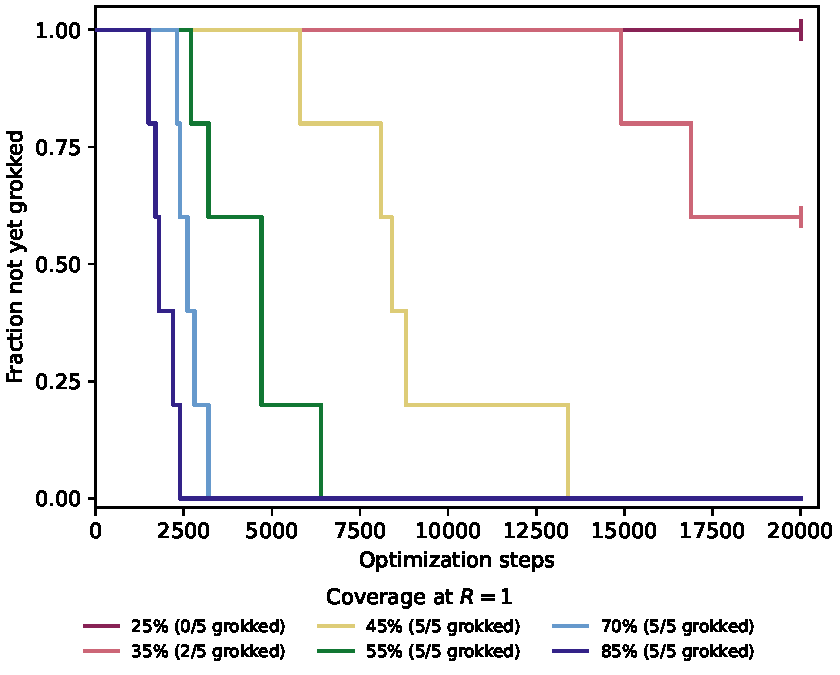
\includegraphics[width=\textwidth]{figs/fig_km_a_R1_by_coverage.pdf}
\caption{\textbf{Kaplan--Meier estimates of time-to-generalization at $R=1$, by coverage.} Curves show the fraction of runs that have not yet reached the 95\% generalization criterion versus optimization steps; ticks mark right-censored runs and legend entries give grokked runs of five. Censoring is total at 25\% coverage (curve flat at 1) and heavy at 35\%. Kaplan--Meier estimates for the repetition arms appear in Fig.~\ref{fig:kmrep} (Appendix~\ref{app:kmrep}).}
\label{fig:km}
\end{figure}

\subsection{Coverage determines whether and when generalization emerges}
\label{sec:coverage}

We first examine the coverage effect at no repetition ($R=1$; the two modes coincide there). Training accuracy reaches 95\% within 100--200 steps at every coverage, and across all 135 runs in the design, \memtime{} never exceeds 500 steps (median 200); every condition enters the memorized regime almost immediately, so the factor space acts on the post-memorization transition rather than on the ability to fit the training set. Test accuracy then separates the coverages (Fig.~\ref{fig:coverage}): median \groktime{} is $1{,}800$ steps at 85\% (IQR $1{,}700$--$2{,}200$), $2{,}600$ at 70\%, $4{,}700$ at 55\%, and $8{,}400$ at 45\%. At 35\% coverage two of five seeds generalize (at $14{,}900$ and $16{,}900$ steps) and three are censored; across all seven 35\%-coverage conditions (35 runs, all repetition levels), three runs in total generalize. At 25\% coverage all five $R=1$ seeds remain below 20\% test accuracy at budget exhaustion (median final accuracy $13.4\%$) despite fully memorized training sets (Fig.~\ref{fig:coverage}d).

The 85\%-versus-45\% contrast is decisive under rank statistics: the median \groktime{} difference is $-6{,}600$ steps (95\% CI $[-11{,}600, -4{,}000]$; rank-biserial $r=+1.0$; exact permutation $p=0.008$, Holm-adjusted $p=0.016$). The censoring-aware survival analyses agree (Fig.~\ref{fig:km}): the permutation log-rank test gives $p=0.008$ for 85\% versus 45\%, and likewise for 85\% versus 25\%, where all five low-coverage runs are censored at the budget (entering censored runs at the worst rank, the exact rank test also gives $p=0.008$, Holm-adjusted $p=0.016$); across all six coverages jointly, the log-rank statistic is $63.1$ on five degrees of freedom ($p < 10^{-4}$; 10{,}000 permutations). Restricted mean time-to-generalization within the 20{,}000-step horizon is $1{,}920$ steps at 85\% coverage, $2{,}660$ at 70\%, $4{,}340$ at 55\%, $8{,}900$ at 45\%, $18{,}360$ at 35\%, and $20{,}000$ at 25\% (no events within the horizon). Within the fixed budget, the number of distinct training problems gates whether and when the transition occurs, whereas the speed of memorization is coverage-insensitive across the entire range tested.

\subsection{Blocked repetition: no detectable effect on the transition at matched dose}
\label{sec:blocked}

At 55\% coverage, median \groktime{} is $4{,}700$ steps at $R=1$, $4{,}200$ at $R=2$, $4{,}400$ at $R=4$, and $3{,}800$ at $R=8$ (blocked; Fig.~\ref{fig:repetition}a,b). The declared family contrasts give median differences of $+300$ steps (95\% CI $[-2{,}600, +2{,}000]$; $p=0.65$) for $R=1$ versus $R=4$ and $+900$ steps (95\% CI $[-1{,}500, +2{,}600]$; $p=0.79$) for $R=1$ versus $R=8$; at 85\% coverage both contrasts are $+100$ steps (CIs $[-500, +700]$ and $[-400, +700]$; $p=0.67$ and $p=0.56$). No contrast survives Holm correction within the family (all Holm-adjusted $p=1.0$), every confidence interval includes zero, and the rank-biserial effect sizes ($|r| \leq 0.28$) are far from the perfect separation produced by the coverage factor ($|r|=1.0$). The censoring-aware analyses agree: pairwise permutation log-rank tests give $p = 0.47$--$0.67$ (55\% and 85\% coverage), the RMST difference for $R=1$ versus $R=8$ is $+280$ steps at 55\% coverage (95\% CI $[-1{,}260, +1{,}700]$) and $+160$ steps at 85\% (95\% CI $[-200, +520]$), and a coverage-stratified Cox model pooling blocked $R \in \{2,4,8\}$ against $R=1$ gives a hazard ratio of $0.96$ (95\% CI $[0.48, 1.94]$; the 35\%-coverage stratum contributes only 3 of 43 events, so the common-hazard assumption is fragile and we do not lean on this estimate). These are null results with bounds: at 85\% coverage the $R=1$-versus-$R=8$ interval $[-400, +700]$ steps excludes repetition-induced shifts larger than roughly $700$ steps earlier (about $39\%$ of the $R=1$ median of $1{,}800$ steps) or $400$ steps later (about $22\%$), and at 55\% the interval $[-1{,}500, +2{,}600]$ excludes shifts larger than roughly $2{,}600$ steps earlier (about $55\%$ of the $4{,}700$-step median) or $1{,}500$ steps later (about $32\%$). The equivalence analysis is a post hoc sensitivity analysis over the grid of margins run ($\pm 10\%$, $\pm 25\%$, and $\pm 50\%$; ratios 1.10, 1.25, and 1.50), and no equivalence claim is made at any margin: on $\log_{10}$ \groktime{} in the uncensored cells, TOST at a $\pm 25\%$ margin (ratio 1.25) would declare equivalence for one of twelve within-mode contrasts, the smallest margin at which equivalence would be declared ranges from 1.21 to 1.87 across contrasts, and with five seeds per group the design has 80\% power only for true ratios of about two or larger. The bounds derive from percentile-bootstrap intervals over five tied, 100-step-resolution values per group and are indicative rather than precise; we do not interpret the null as evidence of exact equivalence.

In the transition zone (35\% coverage), blocked repetition does not tip the balance: $R=2$ yields one generalizing seed of five (at $11{,}900$ steps), and $R=4$ and $R=8$ yield none, with final test accuracies of 32--68\% (medians 36.0\% and 44.5\%) while training accuracy is saturated. Raising $R$ does produce small, consistent effects on secondary outcomes. Memorization is slightly delayed: median \memtime{} rises from 100 to 200 steps at 35\% coverage, from 100 to 300 at 55\%, and from 200 to 500 at 85\% between $R=1$ and $R=8$ (exact rank test $p=0.008$ at each coverage, Holm-adjusted $p=0.048$; Jonckheere--Terpstra trend across $R$ within each coverage: Holm-adjusted $p \leq 0.0003$; exploratory). Sub-critical final accuracy at 25\% coverage is higher with repetition: $13.4\%$ at $R=1$ versus $21.7\%$ at $R=4$ and $21.2\%$ at $R=8$ (blocked; $17.4\%$ at interleaved $R=8$), a measurable improvement over chance ($1/23 = 4.3\%$) that remains far below the 95\% criterion. The within-coverage contrasts are significant under the exact rank test (blocked $R=1$ versus $R=4$: median difference $-8.3$ percentage points, 95\% CI $[-11.3, -4.5]$, $p=0.008$, Holm-adjusted $p=0.024$; $R=1$ versus $R=8$: $p=0.008$), corresponding to a shift from a median of 53 to 86 correct answers among the 397 held-out problems; blocked and interleaved $R=8$ do not differ detectably ($p=0.12$). These secondary-outcome families are exploratory.

\subsection{No detectable difference between interleaved and blocked repetition in GrokTime}
\label{sec:interleaved}

Uniformly reshuffling the repeated copies removes the temporal clustering that blocked repetition introduces, while preserving the multiset and the matched dose. If clustering were the repetition-relevant variable, the modes should diverge; no such divergence is detectable (Fig.~\ref{fig:repetition}c,d). At 55\% coverage, median \groktime{} is $3{,}500$ steps at $R=2$, $4{,}700$ at $R=4$, and $3{,}900$ at $R=8$ interleaved, versus $4{,}200$, $4{,}400$, and $3{,}800$ blocked; at 85\% coverage the interleaved medians are $1{,}800$, $1{,}800$, and $1{,}900$ versus $1{,}700$, $1{,}700$, and $1{,}700$ blocked. Direct mode contrasts at matched $(\coverage, \repetition)$ are all non-significant (exact rank tests: all $p \geq 0.23$; median differences (blocked minus interleaved) within $\pm300$ steps, except $+700$ steps at (55\%, $R=2$) with CI $[-5{,}300, +4{,}300]$), as are the corresponding permutation log-rank tests (all $p \geq 0.39$); the within-interleaved repetition contrasts likewise show no detectable effect (log-rank $p \geq 0.31$; RMST differences within 900 steps at 55\% coverage and 300 at 85\%, all confidence intervals spanning zero). In the transition zone at 35\% coverage no seed generalizes under any interleaved condition. One asymmetry deserves note: sub-critical final accuracy at 35\% coverage is higher under interleaved than blocked repetition (medians $59.6\%$, $55.8\%$, $75.9\%$ at $R=2,4,8$ versus $41.3\%$, $36.0\%$, $44.5\%$), a direction opposite to the clustering hypothesis. The corresponding exploratory tests are non-significant (exact rank tests on the three mode contrasts, Holm-adjusted $p \geq 0.67$), so with five seeds per cell we report the asymmetry as an observation, not an established difference.

\subsection{Below the critical coverage: no detectable rescue by repetition}
\label{sec:below}

At 25\% coverage no run in the design generalizes, with or without repetition, and all runs are censored (0 of 5 seeds in every cell; Clopper--Pearson 95\% CI $[0, 0.52]$ per cell); at 35\% coverage, Fisher exact tests find no detectable effect of repetition level or arrangement on the probability of generalizing (all $p \geq 0.44$), as expected given the event counts (2/5 seeds at $R=1$, 1/5 at $R=2$ blocked, 0/5 elsewhere). The declared extreme contrast compares final test accuracy at (25\%, $R=8$, blocked) with (55\%, $R=1$): a difference of $-75.5$ percentage points (95\% CI $[-78.8, -72.2]$; rank-biserial $r=+1.0$; exact permutation $p=0.008$; the family contains this single contrast, so the Holm-adjusted $p$ is also $0.008$). This contrast varies coverage and repetition simultaneously and should be read as a coverage contrast, not as a test of whether repetition rescues low coverage; the within-coverage comparison (13.4\% at $R=1$ versus 21.2\% at $R=8$, blocked) shows that repetition shifts sub-critical accuracy by single-digit percentage points, while coverage moves the same outcome by more than 80 points across the design.

\subsection{Exploratory: weight-norm dynamics}
\label{sec:wnorm}

At a matched pre-transition step ($1{,}000$), the parameter $\ell_2$ norm differs little across repetition factors and arrangements (medians 23.1--24.3 in every cell; Fig.~\ref{fig:wnorm}a,c): median differences are at most $0.7$ (about 3\% of the norm), and 90\% bootstrap CIs include zero in five of the six contrasts; the one exception ($R=1$ versus $R=2$, blocked, at 55\% coverage) is $+0.53$ with CI $[+0.15, +1.02]$, too small to interpret. With dose held constant, the data arrangement is close to invisible to the optimization trajectory up to the point where the transition would occur. Among the 83 runs that generalize, the final norm does not correlate with \groktime{} (Spearman $\rho = +0.065$, permutation $p = 0.55$; Fig.~\ref{fig:wnorm}b), noting that grokked runs stop at their transition while censored runs continue training, so this comparison mixes stopping times; stratified by coverage, opposing weak associations appear ($\rho = -0.60$ at 85\% with 35 runs, permutation $p = 0.0002$; $+0.29$ at 55\% with 35 runs) that inherit the same stopping-time confound and are not interpreted. The most consistent difference is below the coverage boundary, where all runs reach the full budget and stopping times are matched: at 25\% coverage the median final norm rises from $17.5$ at $R=1$ to $19.4$ at $R=4$ ($p=0.016$, Holm-adjusted $p=0.032$) and $21.0$ at $R=8$ (rank-biserial $r=+1.0$, $p=0.008$, Holm-adjusted $p=0.024$), with the interleaved arrangement in between ($18.3$ at $R=8$; blocked versus interleaved at $R=8$: $p=0.032$). Under the circuit-efficiency reading \citep{varma2024explaining}, memorization consumes weight norm and repetition maintains the memorizing solution's footprint. These comparisons are not part of the declared confirmation families; they are exploratory and are Holm-corrected only within their own small family.

\section{Discussion}

\paragraph{Summary of findings.}
At a matched optimization budget, the two data factors acted on different aspects of learning. Coverage governed whether and when the generalization transition occurred, with a boundary between 35\% and 45\% coverage under our settings: at 35\% coverage three of thirty-five runs generalize across all repetition conditions, at 25\% none do, and median \groktime{} falls monotonically with coverage above the boundary. Repetition, at matched per-example dose, showed no detectable effect on \groktime{} in either arrangement. It was not without effect altogether: raising $R$ delayed memorization by 100--300 steps, raised sub-critical final accuracy at 25\% coverage from $13.4\%$ to about $21\%$, and sustained larger final weight norms there. The pattern is consistent with repetition supporting the memorizing solution while leaving the transition itself governed by unique coverage.

\paragraph{Why a null on \groktime{} is the expected outcome.}
The matched-dose construction explains why the repetition null is expected rather than surprising. With 256 examples per step drawn from a continuously reshuffled stream, interleaved repetition is close to sampling with replacement from the unique set, and blocked repetition mainly changes the number of duplicates within a batch (at $R=8$, as few as 32 unique problems per batch versus up to 256 at $R=1$). The design therefore tests temporal clustering and within-batch duplication; an effect of pure exposure count is excluded by construction, because the dose is matched. What the experiment does not test: repetition under unmatched dose (the practical regime in which more repetition buys more updates); the effect of within-batch diversity per se, which would require a batch-size control arm at matched dose; and repetition beyond the eightfold range. Given this, the appropriate reading of the repetition arm is a bounded statement of the form ``no detectable effect on \groktime{} at matched per-example dose within this design'', not a claim that repetition is generally inert.

\paragraph{Interpretation.}
Under the circuit-efficiency account \citep{varma2024explaining}, grokking reflects competition between an immediately available memorizing circuit and a slower, parameter-efficient generalizing circuit, with weight decay gradually tilting the balance \citep{liu2023omnigrok}. The transition is then driven by the accumulated optimization pressure on the generalizing solution, which our design holds constant across $R$: every condition sees each unique example equally often in expectation, so neither arrangement changes the pressure schedule. For the residual effects we cannot exclude, point estimates of a few hundred steps in either direction with wide intervals, we hypothesize that within-batch duplicates perturb gradient noise without shifting the mean dynamics. The asymmetry at 35\% coverage (higher sub-critical final accuracy under interleaved than blocked repetition) runs opposite to the clustering hypothesis and remains uninterpreted at this sample size; neither arrangement approaches the generalization criterion.

\paragraph{Relation to data-constrained pretraining (speculative).}
A 529-example arithmetic task with a two-layer model is an extreme reduction of pretraining, so the following is speculation, not extrapolation. The results are compatible with the empirical rule that repeating a corpus for a few epochs costs little \citep{muennighoff2023scaling}: at matched step budget, uniform repetition behaves like training on the unique subset, so the cost of data constraint is paid in coverage never bought rather than in interference from the repetition itself. The blocked arm similarly suggests that near-duplicates clustered in time are close to neutral at matched dose. We make no claim that the quantitative coverage boundary measured here (roughly 40\% of the problem space at $20{,}000$ steps) transfers to any other system.

\paragraph{Limitations.}
Six limitations bound the conclusions. First, all results come from a single task family (modular addition, $p=23$), a single architecture and scale, and a single optimizer configuration; the coverage boundary and the size of any repetition effect are expected to move with these choices, including the weight-decay coefficient (1.0), whose large value is part of the standard recipe under which delayed generalization occurs at all. Second, the primary outcome is right-censored at $20{,}000$ steps; runs below the coverage boundary might generalize with larger budgets, so statements about ``no generalization'' are budget-relative. Third, with five seeds per condition the confidence intervals are wide; the bootstrap intervals are computed from five tied, 100-step-resolution values per group and are coarse, and the equivalence analysis is a post hoc sensitivity analysis over margins chosen after the results (at defensible margins the design separates only effects of roughly twofold or larger), so the repetition null is bounded but not equivalence-demonstrating. Fourth, runs stop at the first evaluation step meeting the 95\% criterion, so for grokked runs ``final'' test accuracy is a stopping value rather than a fixed-horizon measurement; the outcome partially reflects the stopping rule. Fifth, test-set size varies with coverage (79 held-out problems at 85\% versus 397 at 25\%), so the 95\% criterion has different granularity across coverage levels and sub-critical accuracies are measured on evaluation sets of different sizes. Sixth, the mechanistic readings are hypothesis-generating: dose was matched by design but within-batch diversity was not, and the weight-norm analysis is exploratory and correlational.

\section{Conclusion}

In a controlled system where every example, exposure, and evaluation is exactly tracked, the transition from memorization to generalization was gated by the coverage of the training distribution rather than by repeated exposure: at matched per-example dose, repetition, whether temporally clustered or uniformly spread, showed no detectable effect on the timing of the transition and did not detectably rescue sub-critical coverage within the $20{,}000$-step budget; it did leave measurable traces on memorization speed, sub-critical accuracy, and weight norms. Within this regime and design, additional unique data changes whether and when the model generalizes, whereas additional repetition at matched per-example dose does not detectably change either.

\section*{Declarations}

\paragraph{Funding.} No funding was received.

\paragraph{Competing interests.} The author has no competing interests.

\paragraph{Ethics approval and consent.} This study is purely computational and involved no human or animal subjects, no personal data, and no human-derived material; no ethics approval or informed consent was required.

\paragraph{Data availability.} The per-run logs (135 runs), the canonical per-run table (\texttt{runs.csv}), the full evaluation history (\texttt{history.csv}), and all analysis outputs (result tables, figures, and the analysis report) are available in a public repository at \url{https://github.com/43aquarius/NeuralProcessingLetters} (tag v1.0.0). The repository is public at the time of submission.

\paragraph{Code availability.} The complete training code, the exact statistical pipeline (enumerated permutation tests, Kaplan--Meier/log-rank/RMST implementation, Fisher and Clopper--Pearson summaries, and the TOST analysis), and the figure scripts are available in the same public repository at \url{https://github.com/43aquarius/NeuralProcessingLetters} (tag v1.0.0). The repository is public at the time of submission.

\paragraph{Author contributions.} Chang Tan (sole author): conceptualization, methodology, software, investigation, formal analysis, data curation, visualization, writing -- original draft, and writing -- review and editing.

\paragraph{Generative AI use.} During the preparation of this work the author used the GLM large-language-model assistant (Z.ai), directed and supervised by the author throughout, at the following stages: drafting and refactoring the experimental and analysis code; planning the statistical analyses; generating the figures and the manuscript tables; inspecting the rendered figures for plotting defects, using the provider's vision-capable model variant; drafting and revising the manuscript text, including language editing; implementing the verification script that re-derives every reported statistic from the archived logs; and checking bibliographic records against public databases. The author designed the study, directed and inspected every analysis, verified the reported numbers against the pipeline outputs, and approved the final content, and takes full responsibility for the content of the publication.

\bibliographystyle{plainnat}
\begin{thebibliography}{20}

\bibitem{allen-zhu2024physics}
Z.~Allen-Zhu and Y.~Li.
\newblock Physics of language models: Part 3.3, knowledge capacity scaling laws.
\newblock In \emph{International Conference on Learning Representations (ICLR)}, 2025.
\newblock Extended abstract; arXiv:2404.05405.

\bibitem{bengio2009curriculum}
Y.~Bengio, J.~Louradour, R.~Collobert, and J.~Weston.
\newblock Curriculum learning.
\newblock In \emph{Proceedings of the 26th International Conference on Machine Learning (ICML)}, pages 41--48, 2009.

\bibitem{hoffmann2022training}
J.~Hoffmann, S.~Borgeaud, A.~Mensch, et~al.
\newblock Training compute-optimal large language models.
\newblock In \emph{Advances in Neural Information Processing Systems (NeurIPS)}, volume 35, pages 30016--30030, 2022.

\bibitem{kaplan2020scaling}
J.~Kaplan, S.~McCandlish, T.~Henighan, et~al.
\newblock Scaling laws for neural language models.
\newblock arXiv preprint arXiv:2001.08361, 2020.

\bibitem{lee2022deduplicating}
K.~Lee, D.~Ippolito, A.~Nystrom, C.~Zhang, D.~Eck, C.~Callison-Burch, and N.~Carlini.
\newblock Deduplicating training data makes language models better.
\newblock In \emph{Proceedings of the 60th Annual Meeting of the Association for Computational Linguistics (ACL)}, pages 8424--8445, 2022.

\bibitem{liu2023omnigrok}
Z.~Liu, E.~J. Michaud, and M.~Tegmark.
\newblock Omnigrok: Grokking beyond algorithmic data.
\newblock In \emph{International Conference on Learning Representations (ICLR)}, 2023.

\bibitem{loshchilov2019decoupled}
I.~Loshchilov and F.~Hutter.
\newblock Decoupled weight decay regularization.
\newblock In \emph{International Conference on Learning Representations (ICLR)}, 2019.

\bibitem{muennighoff2023scaling}
N.~Muennighoff, A.~Rush, B.~Barak, et~al.
\newblock Scaling data-constrained language models.
\newblock In \emph{Advances in Neural Information Processing Systems (NeurIPS)}, volume 36, pages 50358--50376, 2023.

\bibitem{nanda2024progress}
N.~Nanda, L.~Chan, T.~Lieberum, J.~Smith, and J.~Steinhardt.
\newblock Progress measures for grokking via mechanistic interpretability.
\newblock In \emph{International Conference on Learning Representations (ICLR)}, 2023.

\bibitem{power2022grokking}
A.~Power, Y.~Burda, H.~Edwards, I.~Babuschkin, and V.~Misra.
\newblock Grokking: Generalization beyond overfitting on small algorithmic datasets.
\newblock arXiv preprint arXiv:2201.02177, 2022.

\bibitem{vaswani2017attention}
A.~Vaswani, N.~Shazeer, N.~Parmar, et~al.
\newblock Attention is all you need.
\newblock In \emph{Advances in Neural Information Processing Systems (NeurIPS)}, volume 30, 2017.

\bibitem{varma2024explaining}
V.~Varma, R.~Shah, Z.~Kenton, J.~Kram\'{a}r, and R.~Kumar.
\newblock Explaining grokking through circuit efficiency.
\newblock arXiv preprint arXiv:2309.02390, 2023.

\bibitem{wu2021curricula}
X.~Wu, E.~Dyer, and B.~Neyshabur.
\newblock When do curricula work?
\newblock In \emph{International Conference on Learning Representations (ICLR)}, 2021.

\bibitem{zhang2017understanding}
C.~Zhang, S.~Bengio, M.~Hardt, B.~Recht, and O.~Vinyals.
\newblock Understanding deep learning requires rethinking generalization.
\newblock In \emph{International Conference on Learning Representations (ICLR)}, 2017.

\end{thebibliography}

\appendix

\section{Reproducibility details}
\label{app:repro}

\paragraph{Task encoding.}
Problems are the 529 pairs $(a,b) \in \{0,\dots,22\}^2$; the input is the four-token sequence $[a, \texttt{+}, b, \texttt{=}]$ (vocabulary size 25: 23 digits plus the two symbols), and the training target is the answer token at the final position under a causal attention mask. The answer is never part of the input, and the test set is the exact complement of the unique training set for every run. Unique training-set sizes are $n_{\mathrm{uniq}} = \mathrm{round}(\coverage \cdot 529)$: 450 (85\%), 370 (70\%), 291 (55\%), 238 (45\%), 185 (35\%), 132 (25\%), with corresponding test-set sizes 79, 159, 238, 291, 344, 397.

\paragraph{Model and optimizer.}
Two-layer causal transformer: token and positional embeddings, pre-norm blocks with four heads (head dimension 16), GELU MLPs with expansion 4, and a final LayerNorm followed by a linear unembedding. Parameters: 103{,}577. AdamW, learning rate $10^{-3}$, $\beta_1 = 0.9$, $\beta_2 = 0.98$, weight decay 1.0 on all parameters, batch size 256, no gradient clipping, no learning-rate schedule.

\paragraph{Data stream implementation.}
For each run, the seed draws a permutation of the 529 problems; the first $\mathrm{round}(\coverage \cdot 529)$ form the unique training set (the same unique set is shared across $R$ within a seed). Each epoch is a list of $n_{\mathrm{uniq}} \cdot R$ entries (blocked: a shuffled permutation of the unique set with $R$ adjacent copies per example; interleaved: the same multiset fully reshuffled). A single continuous stream concatenates epochs, and consecutive disjoint windows of 256 entries form the batches.

\paragraph{Evaluation and stopping.}
Test and training accuracies are computed every 100 steps on the full evaluation sets with the model in evaluation mode (no dropout is used). \groktime{} (\memtime{}) is the first evaluation step where test (training) accuracy is at least 95\%. A run stops at the first evaluation step where test accuracy reaches 95\%, or at $20{,}000$ steps; ``final'' values are therefore the values at the stopping step.

\paragraph{Software and hardware.}
Python 3.12, PyTorch 2.14 (CPU, one thread per run, two runs in parallel), NumPy 2.1, SciPy 1.14, pandas 2.2, matplotlib 3.9. Two-core CPU, 4\,GB RAM. A censored $20{,}000$-step run takes approximately 8.5 minutes.

\paragraph{Statistical software.}
Exact permutation Mann--Whitney tests with midranks: all $\binom{10}{5}=252$ label assignments enumerated, two-sided $p$-value the proportion of assignments with $|U - n_1 n_2/2|$ at least as large as observed; \texttt{scipy.stats.mannwhitneyu} (two-sided, asymptotic with tie correction) is used only as a numerical cross-check, because SciPy silently substitutes the asymptotic method when ties are present, and the substituted $p$-values can fall below the attainable exact minimum of $2/252 = 0.0079$. Rank-biserial $r = 1 - 2U_1/(n_1 n_2)$, with $U_1$ counting cross-group pairs in which the first-named run has the larger value. Two-group percentile bootstrap CIs of median differences (10{,}000 within-group resamples). Kaplan--Meier estimation, log-rank tests (hypergeometric variance, discrete tied event times), and restricted mean survival time implemented manually; log-rank $p$-values by full enumeration (5-versus-5) or 10{,}000 Monte-Carlo permutations ($k$-sample). Fisher exact tests with Clopper--Pearson intervals. TOST on $\log_{10}$ \groktime{} in permutation and Welch $t$ variants. Jonckheere--Terpstra trend tests across $R$: one-sided (increasing alternative), $p$-values from $10{,}000$ Monte-Carlo permutations of the pooled labels. Spearman rank correlations: two-sided permutation $p$-values from $10{,}000$ permutations of one variable. Stratified Cox model: single binary covariate (blocked $R \in \{2,4,8\}$ versus the shared $R=1$ baseline), stratified by coverage (35, 55, 85\%), Breslow tie handling, Newton--Raphson partial-likelihood fit, Wald 95\% confidence intervals, implemented in NumPy within the archived pipeline (no external survival-analysis package). All randomness from NumPy \texttt{default\_rng} with master seed 20260922 and documented per-analysis offsets.

\section{Deviation log}
\label{app:deviations}

The study design was frozen in an internal design document before the main runs (no public registry entry exists). Deviations from that plan: (i) the maximum step budget was reduced from $40{,}000$ to $20{,}000$ steps based on pilot calibration (85\% coverage groks at approximately $2{,}200$ steps, 45\% at approximately $13{,}400$, and 25\% showed no transition in $15{,}000$ pilot steps), which raises the censored fraction at low coverage; (ii) pilot runs (four conditions, seed 0, $15{,}000$ steps) are used only for calibration and excluded from all analyses; (iii) the analysis families planned in the internal design document refer to coverage and repetition levels that differ from the executed grid: the internal document specifies the top coverage as 100\% (infeasible here, since the test set would be empty) and Family 2 at coverage $\{45,55,70\}$ with $R=1$ versus $R=4$ only, whereas the executed analysis uses 85\% as the top coverage and $\{35,55,85\}$ with both $R=1$ versus $R=4$ and $R=1$ versus $R=8$; (iv) arm D (Table~\ref{tab:design}) was added after implementation revealed that the declared extreme contrast cell (25\%, $R=8$) was missing from the initial run list, with the decision taken after arm-A results were known and before any arm-D data were collected; (v) the two-sample rank test is the enumerated exact permutation Mann--Whitney procedure, adopted in place of SciPy's asymptotic tie-corrected method because the library substitutes that method silently in the presence of ties and it can yield $p$-values below the attainable exact minimum of $2/252$; (vi) the bootstrap confidence intervals of median differences resample within each group, since resampling one group only yields too-narrow intervals, and are percentile intervals rather than the bias-corrected and accelerated (BCa) intervals named in the internal design document (the archived pipeline implements percentile resampling with a fixed random seed); and (vii) the censoring-aware survival analyses (Kaplan--Meier estimation, permutation log-rank tests, restricted mean survival time, and the stratified Cox model), the count-based summaries (Fisher exact tests with Clopper--Pearson intervals), the TOST sensitivity analyses, and the Jonckheere--Terpstra trend tests were not enumerated in the internal design document, which planned only a permutation sensitivity analysis for censored outcomes, exploratory Spearman correlations, and a descriptive trend summary; Methods correspondingly reports these analyses as exploratory or post hoc sensitivity analyses. No data, stopping rule, or family definition was affected.

\section{Descriptive statistics by condition}
\label{app:descriptives}

Table~\ref{tab:descriptives} reports per-condition medians and interquartile ranges across the five seeds, censored-run counts, \memtime{}, and final test accuracy. The main text reports the subset needed for each argument.

\begin{table}[h]
\centering
\caption{\textbf{Descriptive statistics by condition.} \groktime{} (steps, thousands) and final test accuracy are given as median [interquartile range] across $n=5$ seeds; censored runs are counted at the budget ($20{,}000$ steps) in the \groktime{} median. \memtime{} is the median step at which training accuracy first reaches 95\%. Mode is vacuous at $R=1$ (copies coincide); interleaved $R=1$ is identical to blocked $R=1$ and omitted.}
\label{tab:descriptives}
\small
\begin{tabular}{rrlrrrr}
\toprule
Coverage (\%) & $R$ & Mode & GrokTime (k steps) & Cens. & MemTime & Final test acc. (\%) \\
\midrule
25 & 1 & blocked & 20.0 [20.0, 20.0]k & 5/5 & 100 & 13.4 [12.8, 15.6] \\
25 & 4 & blocked & 20.0 [20.0, 20.0]k & 5/5 & 100 & 21.7 [21.2, 21.9] \\
25 & 8 & blocked & 20.0 [20.0, 20.0]k & 5/5 & 200 & 21.2 [19.4, 21.9] \\
25 & 8 & interleaved & 20.0 [20.0, 20.0]k & 5/5 & 100 & 17.4 [17.1, 19.1] \\
35 & 1 & blocked & 20.0 [16.9, 20.0]k & 3/5 & 100 & 90.4 [38.1, 95.1] \\
35 & 2 & blocked & 20.0 [20.0, 20.0]k & 4/5 & 100 & 41.3 [33.4, 44.2] \\
35 & 2 & interleaved & 20.0 [20.0, 20.0]k & 5/5 & 100 & 59.6 [37.5, 62.5] \\
35 & 4 & blocked & 20.0 [20.0, 20.0]k & 5/5 & 200 & 36.0 [33.1, 38.7] \\
35 & 4 & interleaved & 20.0 [20.0, 20.0]k & 5/5 & 100 & 55.8 [32.8, 60.5] \\
35 & 8 & blocked & 20.0 [20.0, 20.0]k & 5/5 & 200 & 44.5 [41.3, 52.3] \\
35 & 8 & interleaved & 20.0 [20.0, 20.0]k & 5/5 & 100 & 75.9 [61.9, 83.7] \\
45 & 1 & blocked & 8.4 [8.1, 8.8]k & 0/5 & 100 & 95.9 [95.5, 96.2] \\
55 & 1 & blocked & 4.7 [3.2, 4.7]k & 0/5 & 100 & 96.6 [95.4, 97.9] \\
55 & 2 & blocked & 4.2 [4.0, 7.2]k & 0/5 & 200 & 96.6 [95.8, 97.5] \\
55 & 2 & interleaved & 3.5 [3.4, 3.8]k & 0/5 & 100 & 96.6 [96.2, 97.1] \\
55 & 4 & blocked & 4.4 [4.0, 5.0]k & 0/5 & 200 & 96.2 [95.8, 96.2] \\
55 & 4 & interleaved & 4.7 [4.0, 6.9]k & 0/5 & 200 & 96.2 [96.2, 96.2] \\
55 & 8 & blocked & 3.8 [3.3, 3.9]k & 0/5 & 300 & 97.1 [95.8, 97.9] \\
55 & 8 & interleaved & 3.9 [3.9, 4.5]k & 0/5 & 200 & 95.8 [95.4, 96.2] \\
70 & 1 & blocked & 2.6 [2.4, 2.8]k & 0/5 & 200 & 96.9 [96.9, 97.5] \\
85 & 1 & blocked & 1.8 [1.7, 2.2]k & 0/5 & 200 & 98.7 [97.5, 98.7] \\
85 & 2 & blocked & 1.7 [1.6, 1.8]k & 0/5 & 200 & 96.2 [96.2, 98.7] \\
85 & 2 & interleaved & 1.8 [1.8, 2.0]k & 0/5 & 200 & 98.7 [97.5, 98.7] \\
85 & 4 & blocked & 1.7 [1.6, 1.8]k & 0/5 & 300 & 98.7 [97.5, 98.7] \\
85 & 4 & interleaved & 1.8 [1.7, 1.9]k & 0/5 & 200 & 98.7 [96.2, 100.0] \\
85 & 8 & blocked & 1.7 [1.6, 1.8]k & 0/5 & 500 & 97.5 [96.2, 97.5] \\
85 & 8 & interleaved & 1.9 [1.7, 1.9]k & 0/5 & 200 & 96.2 [96.2, 97.5] \\
\bottomrule
\end{tabular}
\end{table}

\section{Kaplan--Meier estimates for the repetition arms}
\label{app:kmrep}

\begin{figure}[h]
\centering
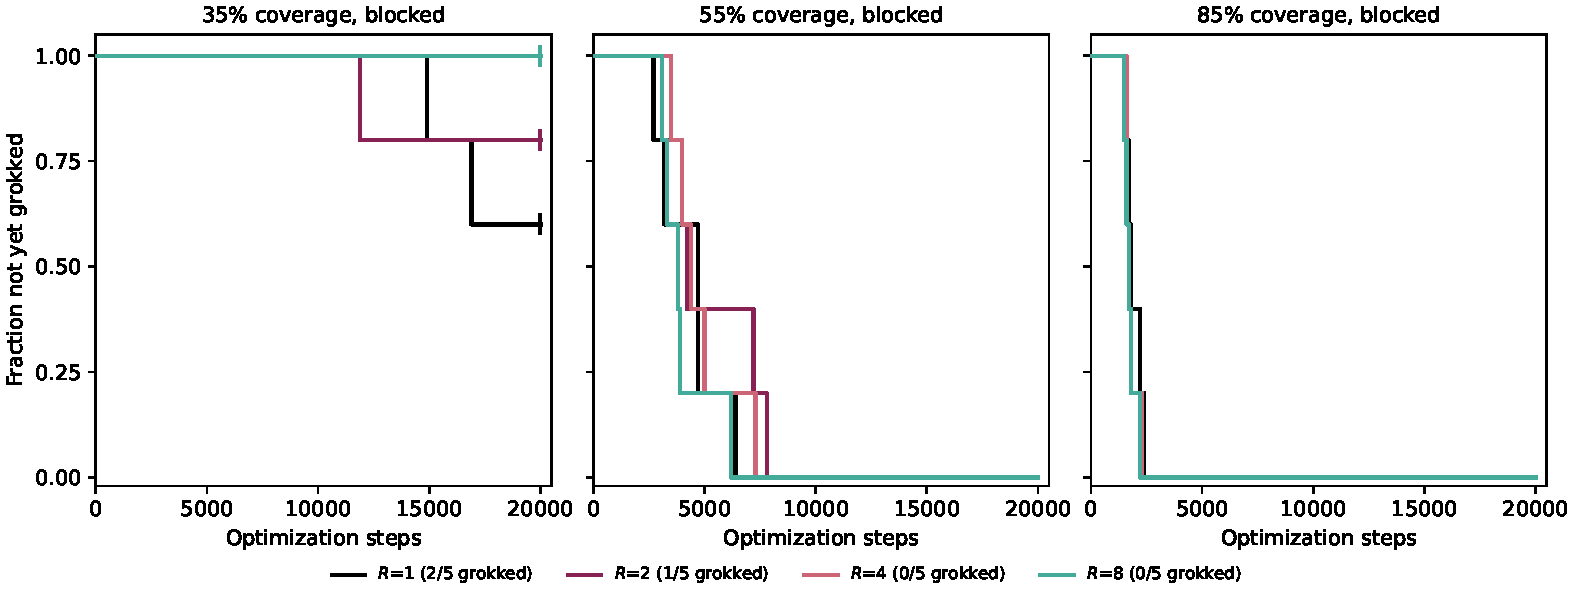
\includegraphics[width=\textwidth]{figs/fig_km_b_blocked.pdf}\\[2pt]
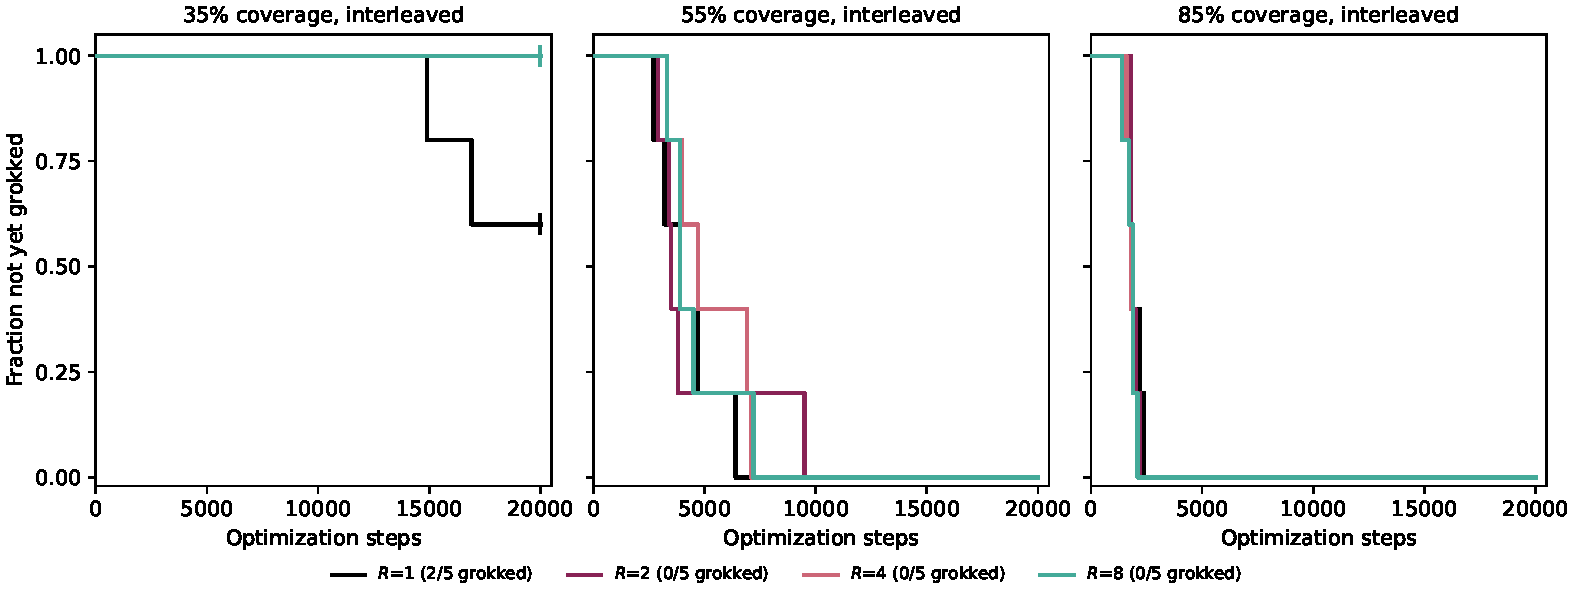
\includegraphics[width=\textwidth]{figs/fig_km_c_interleaved.pdf}
\caption{\textbf{Kaplan--Meier estimates of time-to-generalization under repetition.} (\textbf{top}) Blocked repetition, $R \in \{1,2,4,8\}$, at coverage 35, 55, and 85\% (panels left to right). (\textbf{bottom}) Interleaved repetition, same layout. Curves show the fraction of runs not yet generalized; ticks mark right-censored runs and legend entries give grokked runs of five. At 35\% coverage the curves flatten without dropping, reflecting the near-absence of events; inference there rests on event counts (Fisher exact tests, Sect.~\ref{sec:below}).}
\label{fig:kmrep}
\end{figure}

\end{document}
